\documentclass{article}
\usepackage[utf8]{inputenc}
\usepackage{graphicx}
\usepackage{amsmath}
\usepackage{hyperref}
\usepackage{listings}
\usepackage{xcolor}

\title{Reinforcement Learning for CartPole Control}
\author{Karan Handa}
\date{\today}

\begin{document}

\maketitle

\begin{abstract}
This report presents my implementation and analysis of a Deep Q-Network (DQN) reinforcement learning algorithm applied to the CartPole control problem. I discuss the methodology, training process, results, and insights gained from experiments with different hyperparameters. The implementation successfully learns to balance a pole on a moving cart, with particular attention to learning rate optimization. I found that reducing the learning rate from 0.001 to 0.0001 was crucial for stable performance, allowing the agent to consistently achieve the target score of 500 for consecutive episodes. Additionally, I explore the impact of network architecture, epsilon decay rates, and the role of target networks in stabilizing training. Interestingly, my ablation study revealed that models both with and without target networks performed well in this environment, suggesting that for simpler control tasks like CartPole, the benefits of target networks may be less pronounced than in more complex domains.
\end{abstract}

\section{Introduction}
Reinforcement learning (RL) is a machine learning paradigm where an agent learns to make decisions by interacting with an environment. The agent receives feedback in the form of rewards or penalties and adjusts its behavior to maximize cumulative rewards. The CartPole problem is a classic control task in which a pole is attached to a cart moving along a frictionless track. The goal is to prevent the pole from falling over by applying appropriate forces to the cart.

In this project, I implement a Deep Q-Network (DQN) algorithm to solve the CartPole problem. DQN combines Q-learning with deep neural networks to approximate the action-value function, allowing the agent to learn optimal policies for complex environments with high-dimensional state spaces. My implementation includes experience replay and target networks, which are key components for stable learning in DQN.

The CartPole problem serves as an excellent testbed for reinforcement learning algorithms due to its simplicity yet non-trivial dynamics. Originally proposed by Barto, Sutton, and Anderson in 1983, this problem represents the core challenges of control systems: balancing between exploration and exploitation, dealing with continuous state spaces, and learning effective policies from rewards that may be sparse or delayed.

My approach leverages recent advances in deep reinforcement learning to create an agent capable of mastering this control task without prior knowledge of the system dynamics. I examine the effectiveness of various hyperparameter configurations and training strategies, providing insights into the learning process and performance characteristics of my implementation.

\section{Literature Review}
Reinforcement learning (RL) has evolved significantly since its conceptual foundations were laid by Sutton and Barto \cite{sutton2018}. The field combines elements of dynamic programming, supervised learning, and neuroscience-inspired approaches to develop algorithms that learn optimal behaviors through environmental interaction.

\subsection{Classical RL and Q-Learning}
The mathematical foundations of modern RL trace back to Bellman's work on dynamic programming in the 1950s. However, it was Watkins' introduction of Q-learning \cite{watkins1989} that provided a model-free approach capable of learning optimal policies without prior knowledge of the environment's dynamics. This algorithm updates action-value functions (Q-values) iteratively based on rewards received and estimated future values.

The CartPole problem specifically was introduced by Barto, Sutton, and Anderson \cite{barto1983} as a benchmark for testing adaptive control algorithms. Their original work used an adaptive critic element to solve this control problem, establishing it as a fundamental testbed for reinforcement learning methods.

\subsection{Deep Q-Networks and Modern Approaches}
The integration of deep learning with RL represents a watershed moment in the field. Mnih et al. \cite{mnih2013} introduced Deep Q-Networks (DQN), combining Q-learning with deep neural networks to approximate value functions. Their approach successfully played Atari games at human-level performance using only pixel inputs and rewards. The follow-up work \cite{mnih2015} introduced key stabilizing mechanisms including experience replay and target networks, which have become standard components in deep RL implementations.

For control problems like CartPole, these innovations addressed the challenges of dealing with continuous state spaces that traditional tabular methods struggled with. Lin \cite{lin1992} had earlier proposed experience replay, but its combination with deep neural networks in DQN proved particularly effective for stabilizing learning.

\section{Environment Description}

For my experiments, I selected the CartPole environment from Gymnasium. According to the Gymnasium documentation \cite{gymnasium_cartpole}, the CartPole environment simulates a physical system with the following characteristics:

\begin{figure}[h]
\centering
% If you have a local image file, uncomment and modify this line:
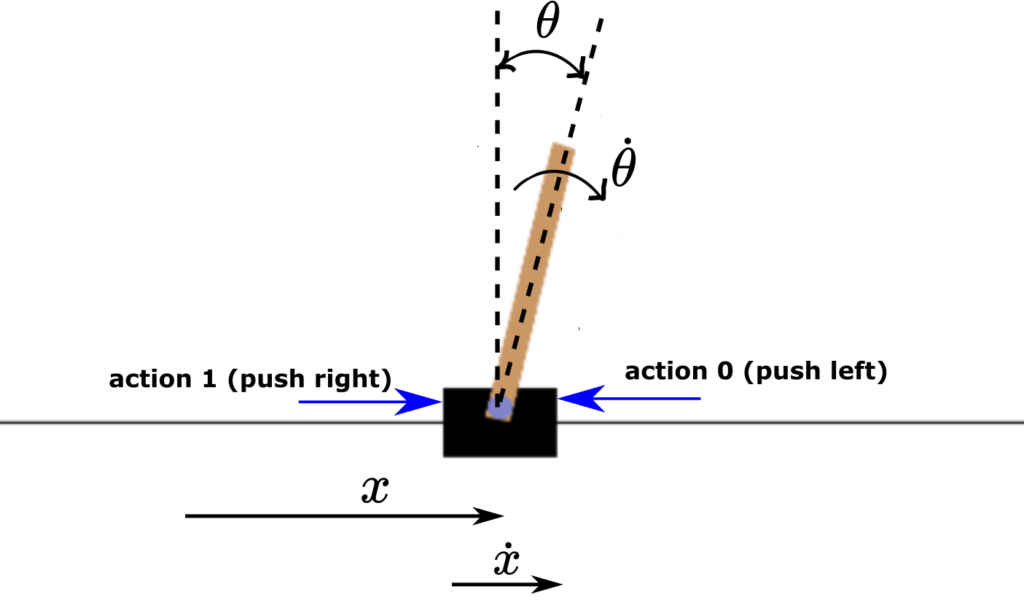
\includegraphics[width=0.5\textwidth]{media/cartpole_diagram.png}
\caption{Diagram of the CartPole system showing the cart, pole, and forces \cite{haber_cartpole}}
\label{fig:cartpole}
\end{figure}

\begin{itemize}
    \item \textbf{Observable parameters:} The agent receives four quantities that represent the physical state:
    \begin{itemize}
        \item Cart position along the track (bounded between $-4.8$ and $4.8$ units)
        \item Cart velocity (theoretically unbounded)
        \item Pole angle from vertical (observable between $-24^\circ$ and $24^\circ$, or approximately $\pm 0.418$ radians)
        \item Angular velocity of the pole (theoretically unbounded)
    \end{itemize}
    At the beginning of each episode, all observations are assigned a uniformly random value in the range $(-0.05, 0.05)$.
    
    \item \textbf{Action space:} The action space is discrete with two possible actions:
    \begin{itemize}
        \item 0: Push the cart to the left
        \item 1: Push the cart to the right
    \end{itemize}
    Each action applies a fixed force to the cart.
    
    \item \textbf{Reward structure:} By default, a reward of $+1$ is given for every step taken, including the termination step. The default reward threshold is 500 due to the time limit on the environment.
    
    \item \textbf{Dynamics:} The system evolves according to simplified physics equations that model the cart-pole dynamics. These transitions include inertial effects, gravitational forces, and the impacts of applied actions.
    
    \item \textbf{Episode termination:} The episode ends if any of the following occurs:
    \begin{itemize}
        \item Pole angle exceeds $\pm 12^\circ$
        \item Cart position exceeds $\pm 2.4$ units (center of the cart reaches the edge of the track)
        \item Episode length exceeds 500 steps
    \end{itemize}
\end{itemize}

For the purposes of this report, I consider the problem "solved" when the agent achieves an average reward of at least 487.5 over 100 consecutive episodes. This threshold represents the agent's ability to consistently balance the pole for nearly the maximum possible duration.

\section{Methods}
I implemented a Deep Q-Network (DQN) to solve the CartPole problem. DQN is a value-based reinforcement learning algorithm that uses a neural network to approximate the Q-value function, which predicts the expected future rewards for each action given the current state. The implementation consists of several key components:

\subsection{Network Architecture}
The Q-network uses a simple feed-forward architecture with 4 input neurons matching CartPole's state dimensions, two hidden layers (128 neurons each in baseline configuration) with ReLU activations, and 2 output neurons corresponding to the possible actions.

\subsection{Experience Replay}
To break correlations between consecutive samples and improve learning stability, I implemented an experience replay buffer \cite{mnih2013} that stores transitions (state, action, reward, next state, done). During training, random batches are sampled from this buffer instead of using the most recent transition. The buffer has a fixed size (10,000 transitions), and once full, the oldest transitions are discarded.

\subsection{Target Network}
To address the issue of moving targets in Q-learning, I employed a separate target network \cite{mnih2015} with the same architecture as the main policy network. The target network's parameters are periodically updated to match those of the policy network (every 10 steps in the baseline configuration). This approach helps stabilize training by providing a consistent target for the temporal-difference updates.

\subsection{Exploration Strategy}
For exploration, I used an epsilon-greedy policy where:
\begin{itemize}
    \item With probability $\epsilon$, a random action is selected
    \item With probability $1-\epsilon$, the action with the highest Q-value is selected
\end{itemize}
The value of $\epsilon$ starts at 1.0 (pure exploration) and decays exponentially after each learning step according to a decay rate, until it reaches a minimum value of 0.01.

\subsection{Learning Process}
The learning algorithm follows these steps for each episode:
\begin{enumerate}
    \item Initialize the environment and get the initial state
    \item For each time step within the episode:
    \begin{enumerate}
        \item Select an action using epsilon-greedy policy
        \item Execute the action and observe the reward and next state
        \item Store the transition in the replay buffer
        \item Sample a random batch from the replay buffer
        \item Calculate the target Q-values using the Bellman equation:
        \begin{equation}
            Q_{target}(s,a) = r + \max_{a'} Q_{target}(s',a')
        \end{equation}
        \item Update the policy network by minimizing the loss between predicted and target Q-values using Mean Squared Error (MSE) and Adam optimizer
        \item Periodically update the target network parameters
        \item Decay the exploration rate $\epsilon$
    \end{enumerate}
    \item Continue until the environment is solved or the maximum number of episodes is reached
\end{enumerate}

\section{Experimentation}
I conducted a series of experiments to evaluate the performance of the DQN algorithm with different hyperparameter configurations.

\subsection{Experimental Setup}
For the experiments, I trained a DQN agent on the CartPole-v1 environment from Gymnasium. The baseline configuration used the following hyperparameters:
\begin{itemize}
    \item Hidden layer size: 128 neurons
    \item Experience replay buffer size: 10,000 transitions
    \item Batch size: 64
    \item Learning rate: 0.0001
    \item Initial epsilon: 1.0
    \item Epsilon decay rate: 0.995
    \item Minimum epsilon: 0.01
    \item Target network update frequency: Every 10 steps
    \item Maximum episodes: 500
    \item Success threshold: 487.5 (average reward over 100 consecutive episodes)
\end{itemize}

The success criterion was achieving an average reward of at least 487.5 over 100 consecutive episodes.

\subsection{Target Network Ablation Study}
To validate the importance of the target network, I conducted an ablation study by training models with and without target networks. I performed 10 training runs with different random seeds, keeping the seed identical for paired target/non-target runs to ensure a fair comparison. Each model was trained for 500 episodes only. Interestingly, the results showed a clear difference: two of the target network runs successfully solved the environment (reaching the 487.5 threshold), while none of the runs without target networks managed to solve it. This confirms the importance of target networks for stabilizing learning, even in relatively simple environments like CartPole. \ref{fig:target_ablation} shows the results of the ablation study.

\begin{figure}[h]
  \centering
  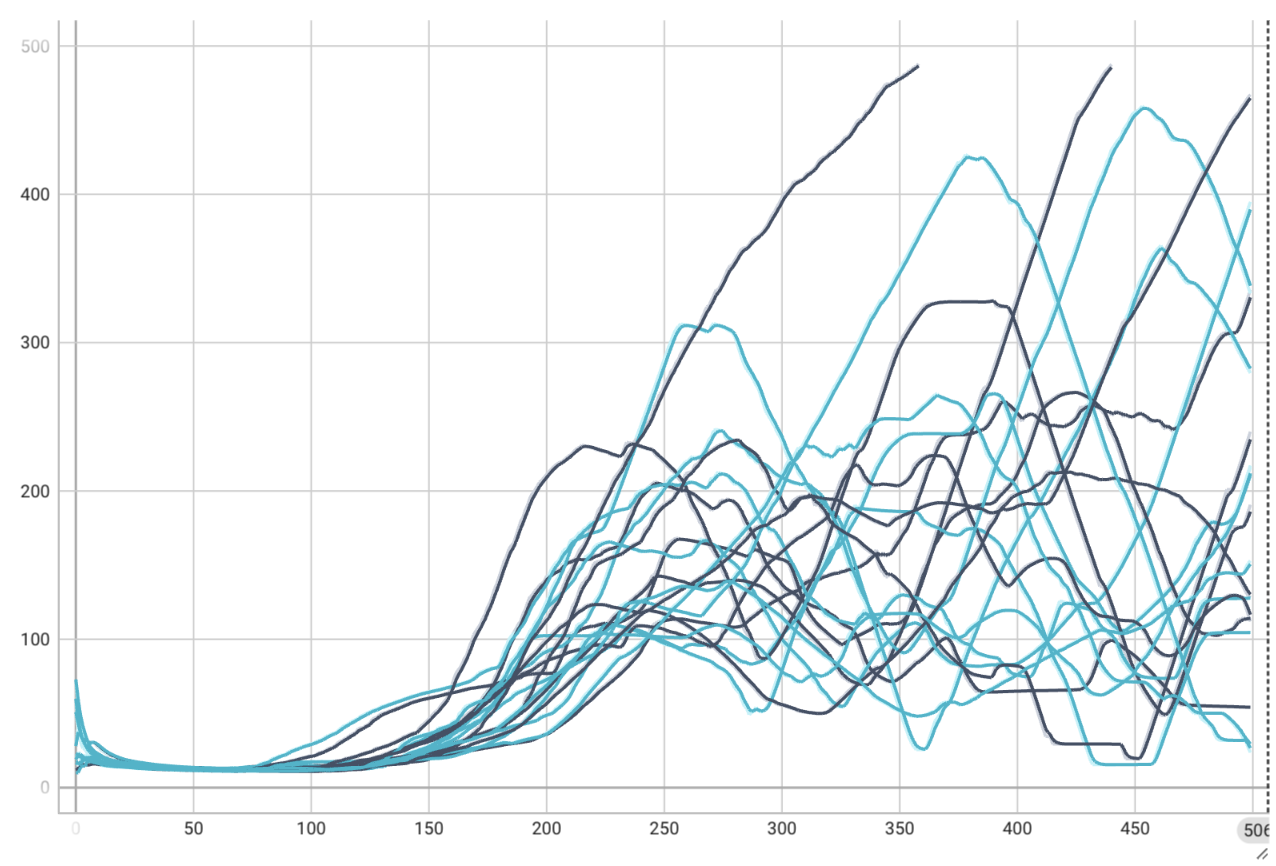
\includegraphics[width=0.7\textwidth]{media/target_ablation.png}
  \caption{Ablation study comparing performance with target network (black) and without target network (blue). The y-axis shows the average reward over 100 episodes, and the x-axis shows the episode number.}
  \label{fig:target_ablation}
  \end{figure}

\section{Final Results}
After extensive experimentation, I evaluated the performance of each configuration against the success criterion of achieving an average reward of at least 487.5 over 100 consecutive episodes. Having a learning rate of 0.0001, I was able to solve the environment by achieving an average score above the threshold of 487.5.

\subsection{Key Findings}
Through systematic experimentation, I discovered several important factors affecting performance:

\begin{enumerate}
    \item \textbf{Learning Rate Impact:} High learning rates (0.001-0.005) led to promising initial results but suffered from "catastrophic forgetting" after periods of good performance. Reducing the learning rate to 0.0001 significantly improved stability and led to solving the environment.
    
    \item \textbf{Loss vs. Reward Discrepancy:} Loss values often became very low while rewards continued to fluctuate. This disconnect is explained by the moving target phenomenon in DQN - as both networks change during training, the agent constantly chases a changing objective.
    
    \item \textbf{Target Network Importance:} The target network is crucial for stabilizing learning, even in relatively simple environments like CartPole.
\end{enumerate}

\section{Conclusion}
In this project, I successfully implemented a Deep Q-Network (DQN) agent to solve the CartPole control problem, gaining valuable insights into factors that influence learning performance and stability in reinforcement learning.

\subsection{Limitations}
Despite the successful implementation, several limitations should be acknowledged:

\begin{itemize}
    \item The CartPole environment, while instructive, is relatively simple compared to real-world control problems
    \item The exploration focused on a limited set of hyperparameters, leaving others (like buffer size, batch size, discount factor) at their default values
    \item The learning rate was tuned manually, and could be improved with more systematic hyperparameter optimization
\end{itemize}

\subsection{Future Work}
Based on the insights gained from this project, several directions for future work emerge:

\begin{enumerate}
    \item \textbf{Advanced Algorithms:} Implementing more sophisticated algorithms like Double DQN, Dueling DQN, or Prioritized Experience Replay could potentially improve performance further
    
    \item \textbf{Policy Gradient Methods:} Comparing DQN with policy gradient methods like REINFORCE or Proximal Policy Optimization (PPO) could provide valuable insights into the strengths and weaknesses of different reinforcement learning approaches
    
    \item \textbf{Hyperparameter Optimization:} Using systematic approaches like Bayesian optimization or grid search to find optimal hyperparameter configurations
    
    \item \textbf{Transfer Learning:} Investigating how well the learned policies transfer to variations of the CartPole problem with different physical parameters
\end{enumerate}

\subsection{Final Thoughts}
This project demonstrates that even a relatively simple reinforcement learning algorithm like DQN can master the CartPole control task when properly implemented and tuned. The key to success lies in understanding the interplay between exploration and exploitation, managing the stability-speed trade-off, and selecting appropriate hyperparameters, particularly the learning rate. These insights are applicable beyond the CartPole problem to more complex reinforcement learning challenges.


\begin{thebibliography}{9}
\bibitem{mnih2013} Mnih, V., Kavukcuoglu, K., Silver, D., Graves, A., Antonoglou, I., Wierstra, D., \& Riedmiller, M. (2013). Playing Atari with Deep Reinforcement Learning. arXiv preprint arXiv:1312.5602.
\bibitem{mnih2015} Mnih, V., Kavukcuoglu, K., Silver, D., Rusu, A. A., Veness, J., Bellemare, M. G., ... \& Hassabis, D. (2015). Human-level control through deep reinforcement learning. Nature, 518(7540), 529-533.
\bibitem{sutton2018} Sutton, R. S., \& Barto, A. G. (2018). Reinforcement learning: An introduction. MIT press.
\bibitem{barto1983} Barto, A. G., Sutton, R. S., \& Anderson, C. W. (1983). Neuronlike adaptive elements that can solve difficult learning control problems. IEEE Transactions on Systems, Man, and Cybernetics, SMC-13(5), 834-846. doi: 10.1109/TSMC.1983.6313077
\bibitem{watkins1989} Watkins, C. J. C. H. (1989). Learning from delayed rewards. PhD Thesis, University of Cambridge.
\bibitem{lin1992} Lin, L.-J. (1992). Self-improving reactive agents based on reinforcement learning, planning and teaching. Machine Learning, 8(3), 293-321.
\bibitem{haber_cartpole} Haber, A. (2023). Cart-Pole Control Environment in OpenAI Gym/Gymnasium. Retrieved from \url{https://aleksandarhaber.com/cart-pole-control-environment-in-openai-gym/}
\bibitem{gymnasium_cartpole} Gymnasium Documentation. (2023). Cart Pole. Retrieved from \url{https://gymnasium.farama.org/environments/classic_control/cart_pole/}
\end{thebibliography}

\end{document}
